\documentclass{article}
\usepackage{graphicx}
\author{Matthew Mosley, Trey Sanchez}
\title{WBAN for Android Documentation}
\begin{document}
\maketitle

\section{Usage}
The WBAN application performs the following functions:

\begin{itemize}
\item plot data in real time
\item display historical data
\item allow user to email data
\item stores data in a comma separated file
\end{itemize}

When the user starts up the app, he will see the start screen shown in Figure \ref{fig:start}.
\begin{figure}[!h]
\label{fig:start}
  \centering
  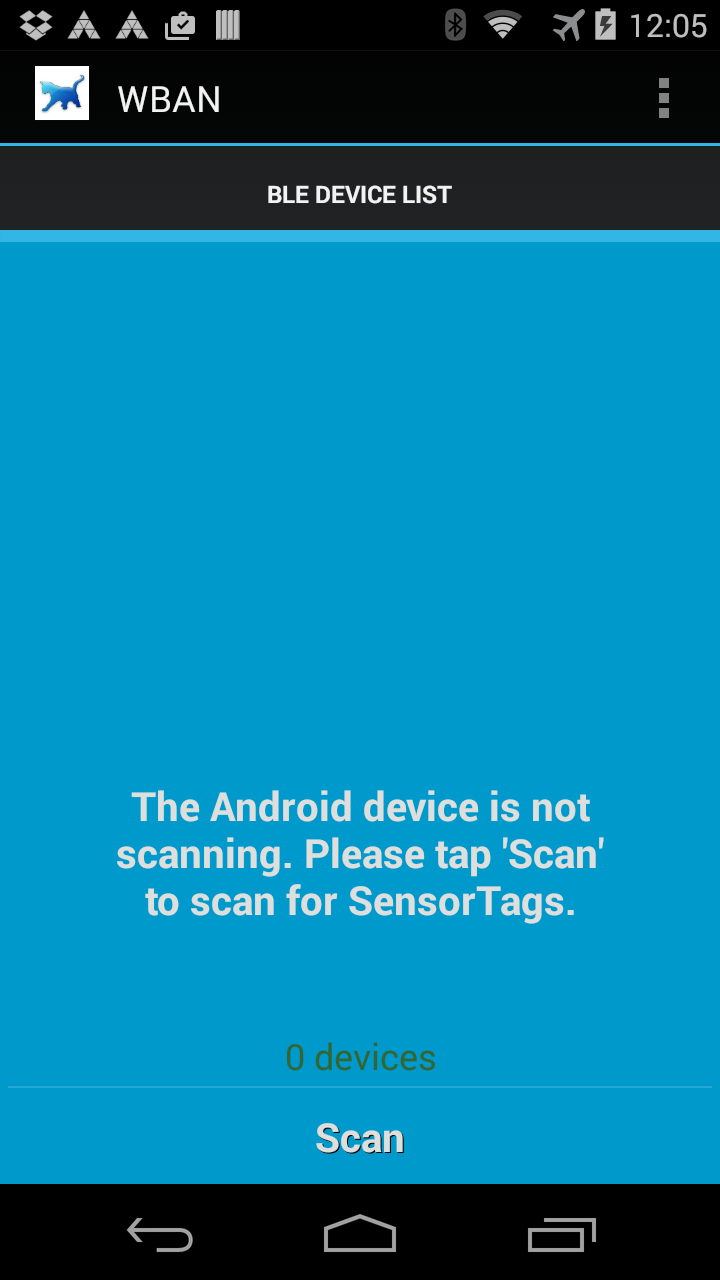
\includegraphics[width=1.7in]{pics/start.png}
  \caption{Start screen}
\end{figure}

The user should press the scan button and the app will use the phone's bluetooth adapter to scan for devices. When
it finds the sensor tag, it will display as in Figure \ref{fig:scan}.

\begin{figure}[!h]
  \centering
  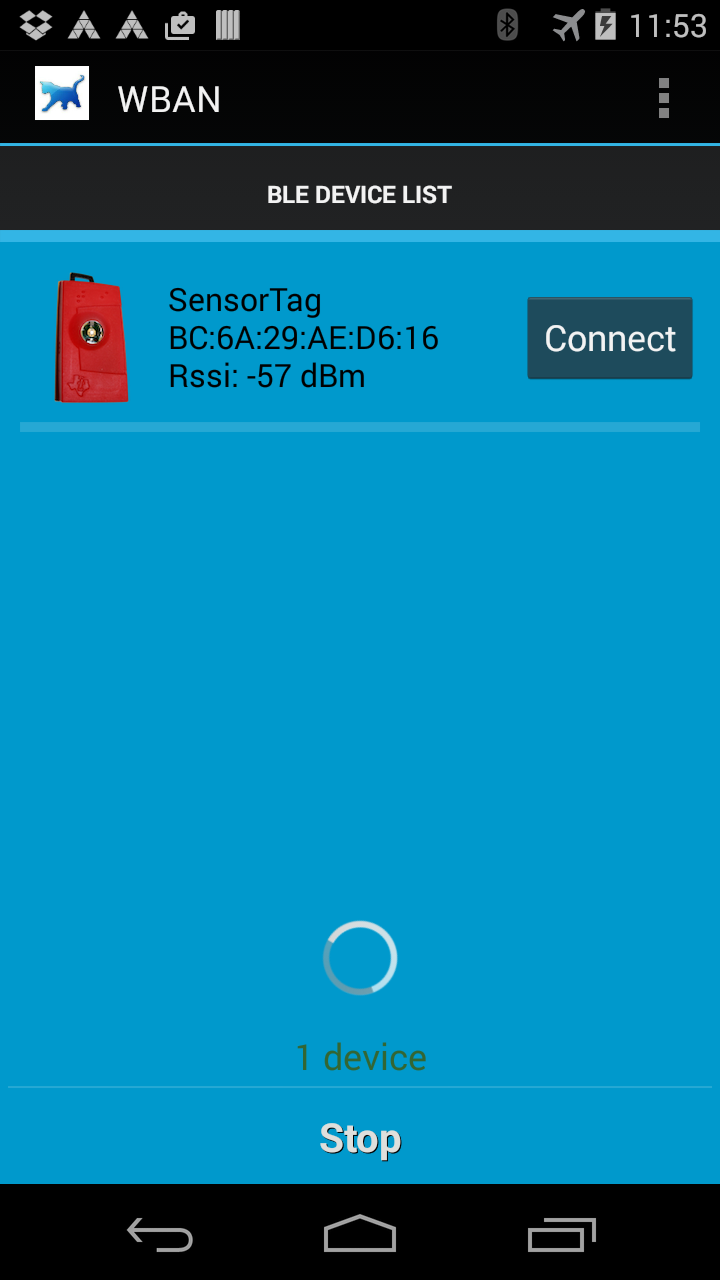
\includegraphics[width=1.7in]{pics/scan.png}
  \caption{Device detected}
  \label{fig:scan}
\end{figure}

The user then presses ``Connect'' and is then taken to the start screen.


\section{Developer Notes}
The WBAN application allows additional sensors to be added (e.g., heart rate, temperature). They should be added in
the code here, here and here.

\end{document}